\section{Solution}
\label{sec:solution}
The main problem is non-convex and very difficult to optimize. 
One typical solution is to use cyclic coordinate method (CCM)\cite{GorskiPK07}. 
To be specific, we iteratively optimize the objective function by fixing $\mathbf{S}$ with respect to $\mathbf{\Theta}$ and vice versa. 
The major problem in such approach is that the quality of the solution depends highly on the initialization as it converges to a local minimum. 
To be specific, if we get a good estimation of $\mathbf{S}$, it is relatively easy to get a good solution for $\mathbf{\Theta}$ as the final loss function puts more emphasis on the correct region pair matching and vice versa. 
Thus, we propose a region based joint model on saliency estimation and region matching for training. 

\subsection{Cyclic Coordinate Training}
Our pipeline is composed of five main steps: 

1.	\emph{Image level (weak) label generation.} 
In this step, we generate the weak labels based on GPS information automatically. 
Google Map provides satellite images, as well as street view images, together with their GPS information to users, so that we can download them conveniently as database. 
Figure~\ref{fig:dbregion} (color masked) shows the region that our database for Boston dataset (introduced in Section~\ref{sec:expr}) covers. 
The colored masks are drawn by Google Map automatically, indicating the buildings. 
\begin{figure}[t]
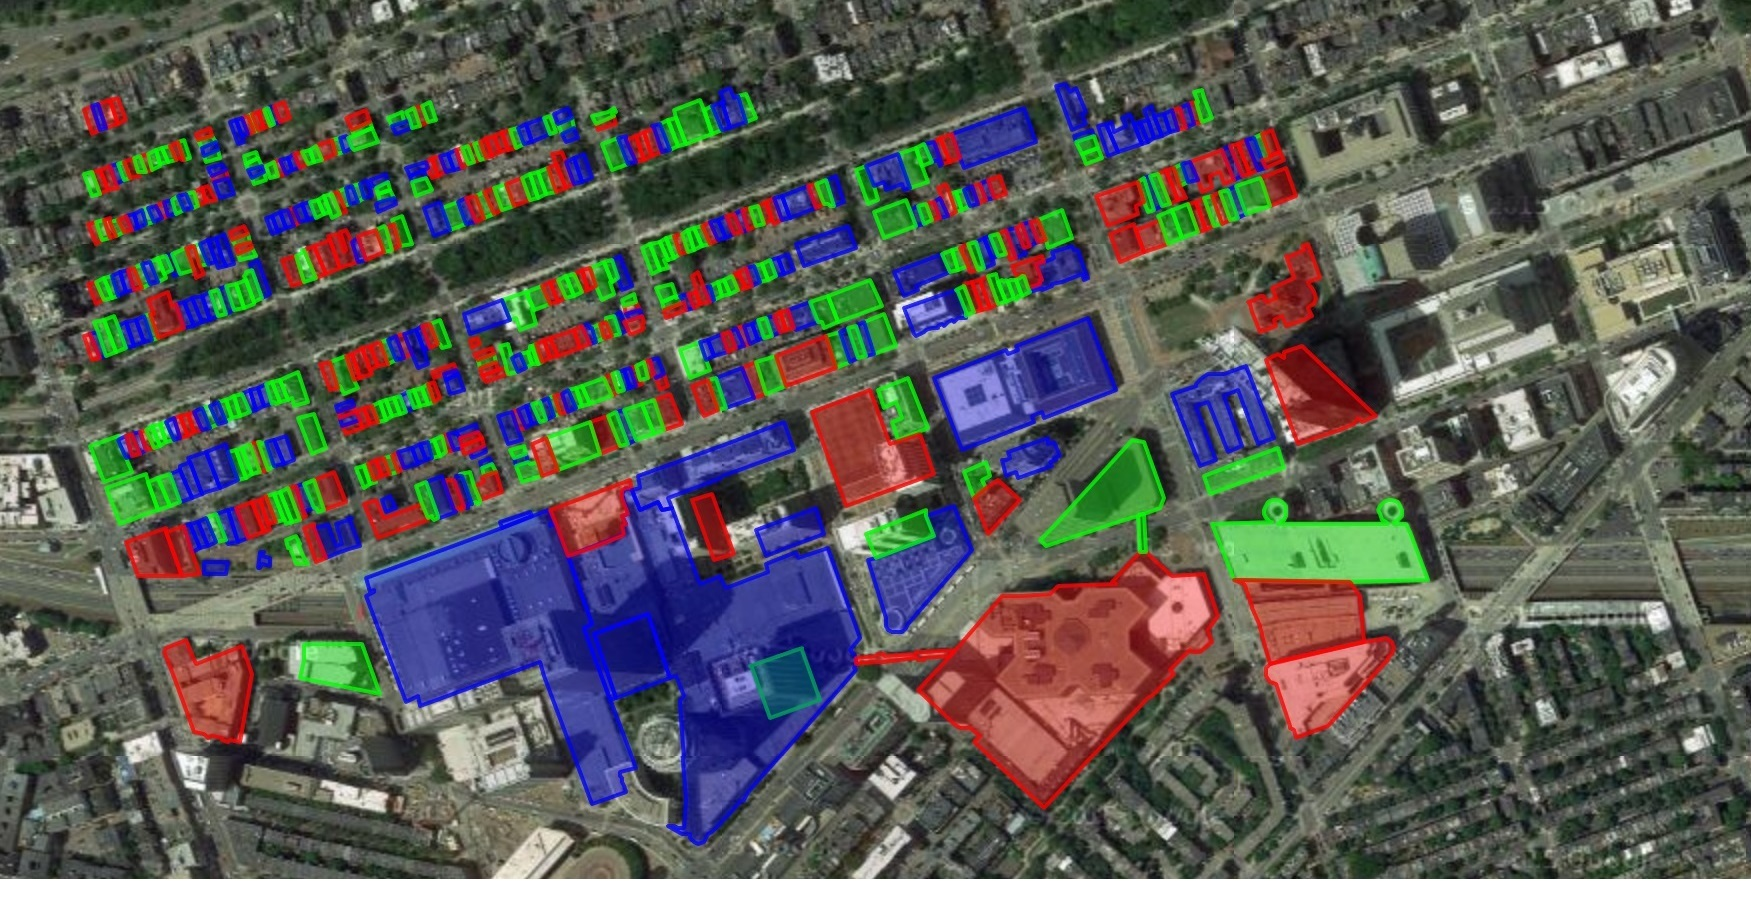
\includegraphics[width=0.7\linewidth]{img/db_region}
\caption{An example for collecting training data with Google Map.}
\label{fig:dbregion}
\end{figure}
After the generation of our database, we sample images in the range that the database covers randomly. 
Google Map provides four different perspectives of view from each point. 
If we just move the sampling point a little, the image with the same perspective would not change a lot. 
Thus, we can get two different images containing almost the same scene, and that is the rationality of our method to generate weak labels automatically.
More specifically, we use Euclidean distance to judge whether two sampling points are near to each other. 
We set the matching label of two images $q, d$ using 
\small
\begin{equation}
\label{eq:weaklabel}
y_{(q, d)} = \left\{
\begin{aligned}
1 \qquad & dist(q,d) \leq \theta \\
0 \qquad & dist(q,d) > \theta
\end{aligned}
\right.
\end{equation}
\normalsize
where $q$ is the sampled image, $d$ is the image from our database, $dist(q,d)$ is the Euclidean distance between the locations of $q$ and $d$ in the real world, $\theta$ is a hyper-parameter that denotes the distance threshold of matching. 
In addition, by zooming, rotating and shifting, we can augment our database to let it contain images with larger diversity. 
Thus, we have completed the generation of training data $D_{train}$.
For database generation, we set $\theta = 25m$.\\[-0.25cm]

2. \emph{Initialization of matching model.}
In this step, we choose a good initialization of matching model. 
The maching model is a weighted Siamese network for region matching as shown in Figure~\ref{fig:siamese}. 
We will elaborate more details in step 4. 
The initialization is done by starting from the degenerate case where the entire image is treated as one region. 
In this case, the region pairs are exactly image pairs $(q, d)$; region pair labels are the exactly image pair labels $y_{(q, d)}$; $w_{ij}$ is set to $1$.
% To be specific, we train a matching model $m(q_i, d_j; \mathbf{\Theta})$ directly using the image pairs. 
% The structure of the network should be the same as that in the following procedure.
% That is, we start from the degenerate case where the entire image is treated as one region.
% In our training procedure, we applied Siamese network for initializing the region matching model. 
% The structure of weighted Siamese network we applied is shown in Figure~\ref{fig:siamese}.
% The CNN is used to extract features from images. 
% In this step,  
% We will introduce more details in \emph{Step 4}.

3. \emph{Saliency Estimation}. Apply the matching model $m(q_i, d_j; \mathbf{\Theta})$ on regions and optimize the main problem with respect to saliency $\mathbf{S}$. This problem can be decomposed to $|Q|+|D|$ separate linear objective quadratic constraint convex optimization problems:
\small
\begin{equation}
\label{eq:decomposed_problem}
\begin{aligned}
& \max_{\mathbf{s}(q)} \sum_{q_i \in q} (m_{i\cdot}^+ - m_{i\cdot}^-) s(q_i) \\
s.t.& ||\mathbf{s}(q)||_2 = 1\\
& s(q_i)\in [0,1]
\end{aligned}
\end{equation}
\normalsize
where
\small
\begin{equation*}
\begin{aligned}
m_{i\cdot}^+& = \sum_{\{d_j|y(q_i,d_j)=1\}} m(q_i,d_j) \\
m_{i\cdot}^-&=\sum_{\{d_j|y(q_i,d_j)=0\}} \min(0, m(q_i,d_j)-\Delta')\\
\end{aligned}
\end{equation*}
\normalsize
We can add the other $|D|$ formulas with respect to $d$ analogously.
This problem has closed form solution:
\small
\begin{equation}
\label{eq:closed_form_solution}
\begin{aligned}
& \mathbf{m}_q = [..., m_{i\cdot }^+ - m_{i\cdot}^-, ...] \geq \mathbf{0} \\
& \hat{\mathbf{s}}(q) = \frac{\mathbf{m}_q}{||\mathbf{m_q}||_2}
\end{aligned}
\end{equation}
\normalsize
Here, $m_{i\cdot }^+, m_{i\cdot}^-$ correspond to the matching status of $q_i$ to regions in positive labels and those in negative labels. 
Note that $m(q_i, d_j)$ is always non-negative due to our constraint in the section of problem formulation, $m_{i\cdot }^+$ is always non-negative and $m_{i\cdot }^-$ is always non-positive. Hence, we have the solution vector  $ \mathbf{m}_q = [..., m_{i\cdot }^+ - m_{i\cdot}^-, ...] \geq \mathbf{0} $. Analogously, we can compute the solution for $\hat{\mathbf{s}}(d)$.

The solution saliency $\hat{\mathbf{S}} = \{\hat{\mathbf{s}}(q)\} \cup \{\hat{\mathbf{s}}(d)\}$ can be used to generate pseudo labels on region level. 
The label is called ``pseudo'' because we fix the parameter $\mathbf{\Theta}$ from an imperfect matching model $m(q_i, d_j; \mathbf{\Theta})$ to get the solution. 

With the hypothesis that different parts of a building would not look very different, if an image pair $(q,d)$ is labelled as matched, then the pair of salient regions $(q_i, d_j)$ with high $s(q_i)$ and $s(d_j)$ should be matched with high level confidence. 
Oppositely,  if an image pair $(q,d)$ is labelled as unmatched, the pair of salient regions $(q_i, d_j)$ with high $s(q_i)$ and $s(d_j)$ should be unmatched with high level confidence, too. 
Thus, we use Eq~\eqref{eq:weight} (i.e. the sum of $s(q_i)$ and $s(d_j)$) to measure the confidence of the pseudo label $y_{(q,d)}$ for region pair $(q_i, d_j)$.
For simplification, here we threshold on the confidence $w_{ij}$ of pseudo label $y_{(q, d)}$ to get positive region pair label. We will give a formal treatment of the mathematical rationale behind thresholding in section~\ref{sec:self_pace}. All the region pairs from negative image pair is considered as negative region pairs. 

4. \emph{Region based matching optimization}. Given the region pair labels generated in step 3, we could rewrite the loss function in eq~\eqref{eq:correspondence} as:
\small
\begin{align}
L(q_i, d_j, y) &= \sum_{y_{(q_i, d_j)} = 1} w_{ij} \cdot y_{(q_i, d_j)}\cdot m(q_i, d_j) + \\
& \sum_{y_{(q_i, d_j)} = 0} w_{ij} (1-y_{(q_i, d_j)})\cdot \max(0, \Delta' - m(q_i,d_j))
\label{eq:region_loss_sum}
\end{align}
\normalsize
, which is actually a pairwise weighted version of the vanilla siamese region matching model. 

5. We repeat step 3 and step 4 and gradually lower the confidence level for the pseudo label as the model becomes more and more accurate and we could rely on more region pair labels generated. 

\begin{figure}[!t]
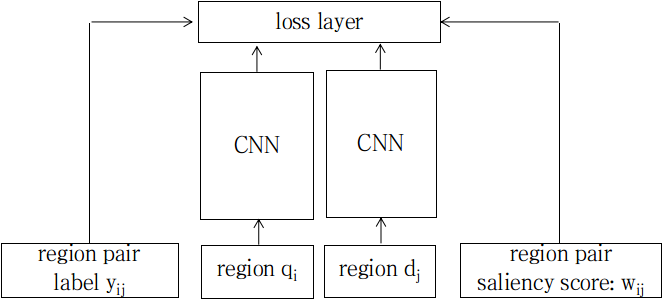
\includegraphics[width=0.9\linewidth]{img/siamese_cj}
\caption{Region matching model in step 4}
\label{fig:siamese}
\end{figure}

\subsection{Self-paced Training}
\label{sec:self_pace}
In fact, the confidence lowering procedure in step 5 could be controlled by a pace function\cite{jiang2015self} on $w_{ij}$ and we could justify the mathematical rationale behind our pipeline by self-paced learning. 
In self-paced learning, a pace function $f(\mathbf{w};k)$ determines a learning scheme, where $k$ increases with the learning step number to control the learning pace. 

In the pace function, it is required that $||\mathbf{w}||_1$ increases with respect to pace step $k$, which means that we'll select more region pairs for training as the learning step number increases. Adding the pace function to the loss function in eq~\eqref{eq:correspondence}, we get:
\small
\begin{equation}
L(q, d, y, k) = \sum_{y_{(q_i, d_j)} = 1} w_{ij}\,L_P(q_i, d_j) + \sum_{y(q_i, d_j) = 0} w_{ij}\,L_N(q_i, d_j) + f(\mathbf{w};k)
\end{equation}
\normalsize
This is the self-paced version loss of the \emph{main problem}. 
Here we use the typical linear scheme pace function:
\begin{equation}
f(\mathbf{w};k) = -\frac{1}{k}||\mathbf{w}||_1
\end{equation}

The solution to the self-paced version doesn't change for steps 1 and 2 as they don't touch the loss function. 
Step 3 has only one minor change in the loss function of its subproblem~\eqref{eq:decomposed_problem}:
\small
\begin{equation}
\max_{\mathbf{s}(q)} \sum_{q_i \in q} (m_{i\cdot}^+ - m_{i\cdot}^- - \underbrace{1 / k}_{\text{change}}) s(q_i)
\end{equation}
\normalsize
Its closed form solution also changes correspondingly:
\small
\begin{equation}
\label{eq:truncate}
\begin{aligned}
m_q^{i} &= \left\{
  \begin{array}{rl}
m_i^+ - m_i^- - \frac{1}{k} & \text{if } m_i^+ - m_i^- > \frac{1}{k}\\
0 & \text{if } m_i^+ - m_i^- <= \frac{1}{k}
  \end{array}\right. \\
\hat{s}(q) &= \frac{m_q}{||m_q||_2}
\end{aligned}
\end{equation}
\normalsize
We see that the solution is actually soft thresholding on the $s(q_i)$. 
We have solution in the same form for $\mathbf{s}(d)$. As $w_{ij} = s(q_i) + s(d_j)$, thresholding on $s(q_i)$ and $s(d_j)$ equals to thresholding on $w_{ij}$. 
Step 4 remains unchanged as it fixes variable $w$. 

In summary, our method can be described as Algorithm~\ref{alg:solution}.
\begin{algorithm}
\begin{algorithmic}[1]  
\REQUIRE{training dataset $D_{train}$, pre-trained matching model parameters $\mathbf{\Theta}$, self-paced function $f$ and stepsize $\mu$}\\
\ENSURE{saliency score $\mathbf{S}$ and region matching model $\mathbf{\Theta^*}$ \\}
~\\
\STATE{Initialize $\mathbf{S}$, $k$ and the matching model $\mathbf{\Theta^* = \Theta}$}
\WHILE{{\sl not converged}}
  \STATE{Estimate saliency score with Eq~\eqref{eq:closed_form_solution}}
  \STATE{Select ``easy'' region level positive labels by thresholding on $s(q_i)$ and $s(d_j)$ using Eq~\eqref{eq:truncate}}
  \STATE{Refine $\mathbf{\Theta^*}$ with the loss function Eq~\eqref{eq:region_loss_sum}}
  \STATE{increase $k$ by $\mu$}
\ENDWHILE
\STATE{\textbf{return} $\mathbf{S}$, $\mathbf{\Theta^*}$}
\end{algorithmic}
\caption{Joint Saliency Estimation and Matching Optimization}
\label{alg:solution}
\end{algorithm}

\subsection{Inference}
After refining the matching model, we propose a corresponding region-based metric to measure the similarity between two images $q$ and $d$, which is 
\begin{equation}
sim_R(q,d) = -\sum_{q_i \in q} \min_{d_j\in d} \frac{|q_i|}{|q|} w_{ij}||f(q_i)-f(d_j)||_2
\label{eq:simR}
\end{equation}
where $|q_i|$ and $|q|$ is the size of region $q_i$ and image $q$, $f(q_i)$ and $f(d_j)$ are the last fully connected layer outputs of CNN in the region matching model. 

Our method of video geo-localization is based on such fact: if a video has not been edited, the geo-location of it should not vary a lot in a short time. 
To find the geo-location of a video, we first retrieve $K$ most similar images in the database for each frame, and collect $K\times F$ images (may overlap) in the database. 
Then, we cluster the images in the database into $C$ clusters, based on their representative vectors in the feature space. 
The video will be localized to the average GPS coordinate of the largest cluster.
